% ------------------------------------------------------------------------ %
% !TEX encoding = UTF-8 Unicode
% !TEX TS-program = pdflatex
% !TEX root = ../Tesi.tex
% !TeX spellcheck = en_US
% ------------------------------------------------------------------------ %
%
% ------------------------------------------------------------------------ %
% 	PROPOSED SOLUTION
% ------------------------------------------------------------------------ %
%
\chapter{Proposed Solution}
%
\label{cap:proposedsolution}
%
% ------------------------------------------------------------------------ %
%
\par In this chapter the development of the solution will be reported step by step, with a full use case. The chapter starts with a list of similar solutions already developed, highlighting the differences between them and my thesis work. The remaining part is composed of tree mains sections: the first explains the choice of the network, the architecture, the naming service, etc. It lays the foundations for the second part: the definition of the Liquid Android middleware, or better the structure of what will do the magic: intercept, encapsulate, spread, and generate distributed intents in the network so made. The two parts are closely related, therefore their relation was taken into account when I made my choice.\\
The real implementation of the valid solution is left for the next chapter.
%

\section{Existing Solutions }
Android distributed systems already exists as specific purposes application to be installed on multiple devices, what it is different to the aim of this thesis work is that these application are closed source projects that can not be reused to build other purposes systems and there is not a coherent framework, library or API to be used to easily build such systems.
I want to give some examples pointing out the nice features have this native distributed Android systems.
\subsection{Boincoid and HTC Power to Give}
Boincoid and HTC Power to Give are Android application which aim is  to exploit Android devices computation power to contribute to scientific discoveries by doing some task. The common idea is to have an Android distributed supercomputer which can handle heavy task and compute tons of data for larger purposes.\\
BOINC is an open-source software platform for computing using volunteered resources \cite{boinc2017open}. It is a program that lets you donate your idle computer time to science projects. Boincoid is a port of the BOINC platform to the Android operating system. The result is an Android BOINC client that behaves exactly like the original one.\\
HTC Power to give is very similar to Boincoid, it is a \textit{CSR (Corporate Social Responsibility)} initiative from HTC that has been jointly developed with Dr. David Anderson at University of California, Berkeley. Using the HTC Power To Give, owners of Android OS smartphones can choose to ‘give back’ by supporting key research projects around the world. Scientific research often requires a vast amount of processing power for data modeling and analysis. HTC Power To Give, supported by the world’s largest single distributed volunteer computing platform BOINC, lets users donate their unused smartphone computing power to science programmes across diverse fields as astronomy, environment, medicine and physics \cite{htc2017power}.
 
\subsection{Plex for Android}
Plex platform is a great, maybe the best, media content streaming distributed system platform. It is mainly composed of two components, the media server, and a client with which enjoy the contents.
\begin{figure}[h]
	\centering
	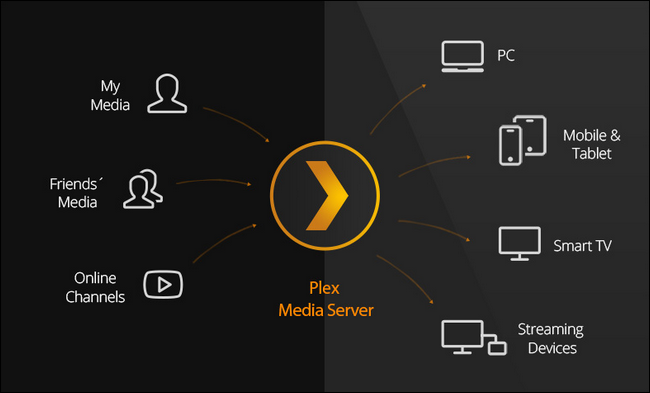
\includegraphics[width=.8\textwidth]{plex}
	\caption{Plex Platform}
	\label{fig:4.1}
\end{figure}
The Plex Media Server either running on Windows, macOS, Linux, FreeBSD or a NAS which organizes audio (music) and visual (photos and videos) content from personal media libraries and streams it to their player counterparts.
The players can either be the Plex Apps available for mobile devices, smart TVs, and streaming boxes, or the web UI of the Plex Media Server called Plex Web App, or the old Plex player called Plex Home Theater.\\
In particular Plex for Android application can connect to the media server to play its content and in addition it can search for Plex players in a LAN and send streamed content such as videos, movies or photo, to another player that can be also an Android device. In this way the Android Plex application client can behave like the Liquid Android system i want to develop. It can send a sort of \textit{Android intent}, to reproduce a media, from one device to another, and then it can send commands such as pause, rewind, forward and so on. The limits of such a system are that it is possible to send, and play, only multimedia contents, and only to devices which have the Plex app activity in foreground on the device.

\subsection{Goolgle Home and Cast API}
Google itself provides an application to control and send contents form an Android device, to some special devices in home network. \textit{Google Home} is an Android application which can find, setup, manage and control, Google's home devices like the \textit{Google Chromecast}. In this way is easy to setup and control and Android distributed system in which user can sent multimedia contents and command to the Google Home devices in the LAN. For these reason Google provides a development library, included in the Android framework, called \textit{Cast API} with which it is easy, for a developer, to build applications that can send multimedia streams to other Google devices specifically built for these purposes.\\
Also in this case the limitation is the kind of content, only multimedia, and also the type of devices involved which are limited number of special purposes devices.

\subsection{DroidMote and Remote control systems }
If we consider the possibility to control remote devices in a LAN, there are actually many different kind of applications that can do that also in an Android environment.
DroidMote is probably the most complete application to control remotely an Android device from another one. It is composed by two parts, the server, to be installed in the device to be controlled, and the client, to be installed in the one which controls. With this application is possible to control entirely the device running the server component: is it possible to open applications, perform tasks, open system settings and so on.\\
These kind of systems are capable to generate local intents in remote devices over a LAN but in a completely different way from I want to develop the solution to the given problem. In this case the \textit{controller} is explicitly controlling the remote device as it is using only the \textit{controlled} one. These systems are solution only to the problem of remote control, they can not exploit distributed Android devices computation power, in fact in an environment like this Android devices are not cooperating to perform task but one of them is only controlling another one.
\section{General Idea}
\section{Network Architecture}


%
% -----------------------------END--------------------------------- %